% Options for packages loaded elsewhere
% Options for packages loaded elsewhere
\PassOptionsToPackage{unicode}{hyperref}
\PassOptionsToPackage{hyphens}{url}
%
\documentclass[
  ignorenonframetext,
  aspectratio=169,
]{beamer}
\newif\ifbibliography
\usepackage{pgfpages}
\setbeamertemplate{caption}[numbered]
\setbeamertemplate{caption label separator}{: }
\setbeamercolor{caption name}{fg=normal text.fg}
\beamertemplatenavigationsymbolsempty
% remove section numbering
\setbeamertemplate{part page}{
  \centering
  \begin{beamercolorbox}[sep=16pt,center]{part title}
    \usebeamerfont{part title}\insertpart\par
  \end{beamercolorbox}
}
\setbeamertemplate{section page}{
  \centering
  \begin{beamercolorbox}[sep=12pt,center]{section title}
    \usebeamerfont{section title}\insertsection\par
  \end{beamercolorbox}
}
\setbeamertemplate{subsection page}{
  \centering
  \begin{beamercolorbox}[sep=8pt,center]{subsection title}
    \usebeamerfont{subsection title}\insertsubsection\par
  \end{beamercolorbox}
}
% Prevent slide breaks in the middle of a paragraph
\widowpenalties 1 10000
\raggedbottom
\AtBeginPart{
  \frame{\partpage}
}
\AtBeginSection{
  \ifbibliography
  \else
    \frame{\sectionpage}
  \fi
}
\AtBeginSubsection{
  \frame{\subsectionpage}
}
\usepackage{iftex}
\ifPDFTeX
  \usepackage[T1]{fontenc}
  \usepackage[utf8]{inputenc}
  \usepackage{textcomp} % provide euro and other symbols
\else % if luatex or xetex
  \usepackage{unicode-math} % this also loads fontspec
  \defaultfontfeatures{Scale=MatchLowercase}
  \defaultfontfeatures[\rmfamily]{Ligatures=TeX,Scale=1}
\fi
\usepackage{lmodern}

\usetheme[]{Boadilla}
\usecolortheme[]{default}
\usefonttheme[]{professionalfonts}
\ifPDFTeX\else
  % xetex/luatex font selection
\fi
% Use upquote if available, for straight quotes in verbatim environments
\IfFileExists{upquote.sty}{\usepackage{upquote}}{}
\IfFileExists{microtype.sty}{% use microtype if available
  \usepackage[]{microtype}
  \UseMicrotypeSet[protrusion]{basicmath} % disable protrusion for tt fonts
}{}
\makeatletter
\@ifundefined{KOMAClassName}{% if non-KOMA class
  \IfFileExists{parskip.sty}{%
    \usepackage{parskip}
  }{% else
    \setlength{\parindent}{0pt}
    \setlength{\parskip}{6pt plus 2pt minus 1pt}}
}{% if KOMA class
  \KOMAoptions{parskip=half}}
\makeatother


\usepackage{longtable,booktabs,array}
\newcounter{none} % for unnumbered tables
\usepackage{calc} % for calculating minipage widths
\usepackage{caption}
% Make caption package work with longtable
\makeatletter
\def\fnum@table{\tablename~\thetable}
\makeatother
\usepackage{graphicx}
\makeatletter
\newsavebox\pandoc@box
\newcommand*\pandocbounded[1]{% scales image to fit in text height/width
  \sbox\pandoc@box{#1}%
  \Gscale@div\@tempa{\textheight}{\dimexpr\ht\pandoc@box+\dp\pandoc@box\relax}%
  \Gscale@div\@tempb{\linewidth}{\wd\pandoc@box}%
  \ifdim\@tempb\p@<\@tempa\p@\let\@tempa\@tempb\fi% select the smaller of both
  \ifdim\@tempa\p@<\p@\scalebox{\@tempa}{\usebox\pandoc@box}%
  \else\usebox{\pandoc@box}%
  \fi%
}
% Set default figure placement to htbp
\def\fps@figure{htbp}
\makeatother





\setlength{\emergencystretch}{3em} % prevent overfull lines

\providecommand{\tightlist}{%
  \setlength{\itemsep}{0pt}\setlength{\parskip}{0pt}}



 


\makeatletter
\@ifpackageloaded{caption}{}{\usepackage{caption}}
\AtBeginDocument{%
\ifdefined\contentsname
  \renewcommand*\contentsname{Table of contents}
\else
  \newcommand\contentsname{Table of contents}
\fi
\ifdefined\listfigurename
  \renewcommand*\listfigurename{List of Figures}
\else
  \newcommand\listfigurename{List of Figures}
\fi
\ifdefined\listtablename
  \renewcommand*\listtablename{List of Tables}
\else
  \newcommand\listtablename{List of Tables}
\fi
\ifdefined\figurename
  \renewcommand*\figurename{Figure}
\else
  \newcommand\figurename{Figure}
\fi
\ifdefined\tablename
  \renewcommand*\tablename{Table}
\else
  \newcommand\tablename{Table}
\fi
}
\@ifpackageloaded{float}{}{\usepackage{float}}
\floatstyle{ruled}
\@ifundefined{c@chapter}{\newfloat{codelisting}{h}{lop}}{\newfloat{codelisting}{h}{lop}[chapter]}
\floatname{codelisting}{Listing}
\newcommand*\listoflistings{\listof{codelisting}{List of Listings}}
\makeatother
\makeatletter
\makeatother
\makeatletter
\@ifpackageloaded{caption}{}{\usepackage{caption}}
\@ifpackageloaded{subcaption}{}{\usepackage{subcaption}}
\makeatother

\usepackage{bookmark}
\IfFileExists{xurl.sty}{\usepackage{xurl}}{} % add URL line breaks if available
\urlstyle{same}
\hypersetup{
  pdftitle={Lecture 2: Discrete-Time Markov Chains},
  hidelinks,
  pdfcreator={LaTeX via pandoc}}


\title{\texorpdfstring{Lecture 2: Discrete-Time Markov
Chains}{Lecture 2: Discrete-Time Markov Chains}}
\author{}
\date{}

\begin{document}
\frame{\titlepage}


\section{Classification of States}\label{classification-of-states}

\begin{frame}{Classification of States}
\protect\phantomsection\label{classification-of-states-1}
So far, we have studied how a Markov chain moves between states and how
to calculate \(n\)-step transition probabilities.

We now ask:

\begin{quote}
\textbf{What does the structure of the chain tell us about its long-run
behaviour?}
\end{quote}

A Markov chain may contain groups of states that the process can leave,
and groups that it cannot leave once entered.

For example, a chain may eventually enter either \({1}\) or \({4,5}\)
and then remain there.

To analyse this structure, we study:

\begin{itemize}
\tightlist
\item
  \textbf{accessibility and communication}; \textbf{communication
  classes};
\item
  \textbf{closed and non-closed classes}; \textbf{transient and
  recurrent states}.
\end{itemize}

Throughout, \(\{X_n\}_{n\geq 0}\) is a time-homogeneous Markov chain
with state space \(S\) and transition matrix \(P=(p_{ij})\).
\end{frame}

\begin{frame}{Applications in Insurance}
\protect\phantomsection\label{applications-in-insurance}
State classification is useful when a Markov chain models the evolution
of an insurance system.

\begin{itemize}
\tightlist
\item
  \textbf{NCD system:} determine whether different premium levels
  communicate and whether there is a single long-run class.
\item
  \textbf{Health insurance:} identify transient health states and closed
  states such as death.
\item
  \textbf{Claims or risk models:} distinguish temporary conditions from
  long-term regimes.
\end{itemize}

The classification helps answer:

\begin{itemize}
\tightlist
\item
  Which states can the process eventually reach?
\item
  Which states can be revisited indefinitely?
\item
  Which states can be left permanently?
\item
  Does the process eventually enter a particular closed class?
\end{itemize}

These questions lead naturally to \textbf{absorption probabilities} and
\textbf{long-run behaviour}.
\end{frame}

\begin{frame}{Accessibility and Communication}
\protect\phantomsection\label{accessibility-and-communication}
For \(i,j\in S\), state \(j\) is \textbf{accessible} from state \(i\),
written \(i\rightarrow j\), if

\[
p_{ij}^{(n)}>0
\]

for some \(n\geq0\).

Thus, starting from \(i\), there is a positive probability of reaching
\(j\) after some number of transitions.

Accessibility does \textbf{not} require a one-step transition.

If there are states \(k_1,\ldots,k_r\) such that

\[
p_{ik_1}p_{k_1k_2}\cdots p_{k_rj}>0,
\]

then \(i\rightarrow j\).
\end{frame}

\begin{frame}{Communication}
\protect\phantomsection\label{communication}
States \(i\) and \(j\) \textbf{communicate}, written
\(i\leftrightarrow j\), if each is accessible from the other:

\[
i\rightarrow j
\quad\text{and}\quad
j\rightarrow i.
\]

Communication is an \textbf{equivalence relation}, so it partitions
\(S\) into \textbf{communication classes}.

Within a communication class, every pair of states communicates.
\end{frame}

\begin{frame}{Closed Classes}
\protect\phantomsection\label{closed-classes}
A communication class \(C\) is \textbf{closed} if, once the chain enters
\(C\), it cannot move to a state outside \(C\).

Equivalently,

\[
p_{ij}=0
\qquad\text{for all }i\in C,\ j\notin C.
\]

A class that is not closed is called a \textbf{non-closed class}.
\end{frame}

\begin{frame}{Absorbing States}
\protect\phantomsection\label{absorbing-states}
A closed class containing a single state is an \textbf{absorbing state}.

State \(i\) is absorbing if

\[
p_{ii}=1.
\]

Thus, once the chain enters an absorbing state, it remains there
forever.
\end{frame}

\begin{frame}{Reducibility}
\protect\phantomsection\label{reducibility}
If the entire state space consists of one communication class, the chain
is \textbf{irreducible}.

Otherwise, it is \textbf{reducible}.

Hence,

\[
\boxed{\text{one communication class}\iff\text{irreducible}.}
\]
\end{frame}

\begin{frame}{Irreducible Markov Chains}
\protect\phantomsection\label{irreducible-markov-chains}
A Markov chain is \textbf{irreducible} if every state can be reached
from every other state.

Equivalently, the entire state space is a single communication class.

Thus, for every \(i,j\in S\),

\[
i\leftrightarrow j.
\]

If \(S\) contains more than one communication class, the Markov chain is
\textbf{reducible}.
\end{frame}

\begin{frame}{Why Is Irreducibility Important?}
\protect\phantomsection\label{why-is-irreducibility-important}
Irreducibility means that no state or group of states is permanently
separated from the others.

For a finite irreducible Markov chain:

\begin{itemize}
\tightlist
\item
  there is a \textbf{unique stationary distribution};
\item
  every state is \textbf{revisited repeatedly} in the long run.
\end{itemize}

Thus, the long-run behaviour of the entire chain can be studied through
a single stationary distribution.
\end{frame}

\begin{frame}{Transient and Recurrent States}
\protect\phantomsection\label{transient-and-recurrent-states}
A state is \textbf{recurrent} if, starting from that state, the chain
returns to it with probability \(1\).

A state is \textbf{transient} if there is a positive probability that
the chain never returns to it.

For a \textbf{finite} Markov chain:

\[
\boxed{
\begin{array}{c}
\text{closed communication class}\\
\Downarrow\\
\text{recurrent states}
\end{array}
}
\qquad
\boxed{
\begin{array}{c}
\text{non-closed communication class}\\
\Downarrow\\
\text{transient states}
\end{array}
}
\]

A non-closed class can eventually be left; a closed class cannot.
\end{frame}

\begin{frame}{Mathematical Definition}
\protect\phantomsection\label{mathematical-definition}
Given \(X_0=i\), define the first return time

\[
T_i=\min\{n\geq1:X_n=i\}.
\]

State \(i\) is \textbf{recurrent} if

\[
\Pr(T_i<\infty\mid X_0=i)=1.
\]

It is \textbf{transient} if

\[
\Pr(T_i<\infty\mid X_0=i)<1.
\]

Thus, recurrence means return with probability \(1\), while transience
means there is a positive probability of never returning.
\end{frame}

\begin{frame}{Key Idea}
\protect\phantomsection\label{key-idea}
The communication structure tells us what can happen in the long run.

{\def\LTcaptype{none} % do not increment counter
\begin{longtable}[]{@{}ll@{}}
\toprule\noalign{}
Structure & Interpretation \\
\midrule\noalign{}
\endhead
\(i\rightarrow j\) & \(j\) is accessible from \(i\) \\
\(i\leftrightarrow j\) & \(i\) and \(j\) communicate \\
Closed class & Cannot be left once entered \\
Non-closed class & Can be left \\
Recurrent state & Returned to with probability \(1\) \\
Transient state & Positive probability of never returning \\
\bottomrule\noalign{}
\end{longtable}
}

For a \textbf{finite} Markov chain:

\[
\boxed{
\text{closed class}\Rightarrow\text{recurrent},
\qquad
\text{non-closed class}\Rightarrow\text{transient}.
}
\]
\end{frame}

\begin{frame}{Example: Five-State Classification}
\protect\phantomsection\label{example-five-state-classification}
Consider a Markov chain with state space \(S={1,2,3,4,5}\) and
transition matrix

\[
P=
\begin{bmatrix}
1&0&0&0&0\\
1/5&1/5&1/5&1/5&1/5\\
1/3&1/3&0&1/3&0\\
0&0&0&0&1\\
0&0&0&1/2&1/2
\end{bmatrix}.
\]

Identify the communication classes, determine which are closed, classify
the states, and determine whether the chain is irreducible.
\end{frame}

\begin{frame}{Five-State Classification}
\protect\phantomsection\label{five-state-classification}
The communication classes are

\[
C_1=\{1\},\qquad
C_2=\{2,3\},\qquad
C_3=\{4,5\}.
\]

\(C_1\) is closed because \(p_{11}=1\).

\(C_3\) is closed because states \(4\) and \(5\) communicate and neither
can leave \({4,5}\).

\(C_2\) is non-closed because states \(2\) and \(3\) communicate, but
the chain can leave the class; for example,

\[
p_{21}>0,\qquad p_{24}>0.
\]

Therefore,
\(\boxed{{1},{4,5}\text{ are closed classes; }{2,3}\text{ is a non-closed class}.}\)
\end{frame}

\begin{frame}{Five-State Classification}
\protect\phantomsection\label{five-state-classification-1}
Since the chain is finite:

\[
\boxed{1,4,5\text{ are recurrent}}
\]

and

\[
\boxed{2,3\text{ are transient}.}
\]

The chain has three communication classes, so it is \textbf{reducible}.

The structure can be summarised as

\[
\{2,3\}
\longrightarrow
\{1\}
\qquad\text{or}\qquad
\{4,5\},
\]

where \({1}\) and \({4,5}\) are closed classes.
\end{frame}

\begin{frame}{State Classification Roadmap}
\protect\phantomsection\label{state-classification-roadmap}
\begin{figure}[H]

{\centering 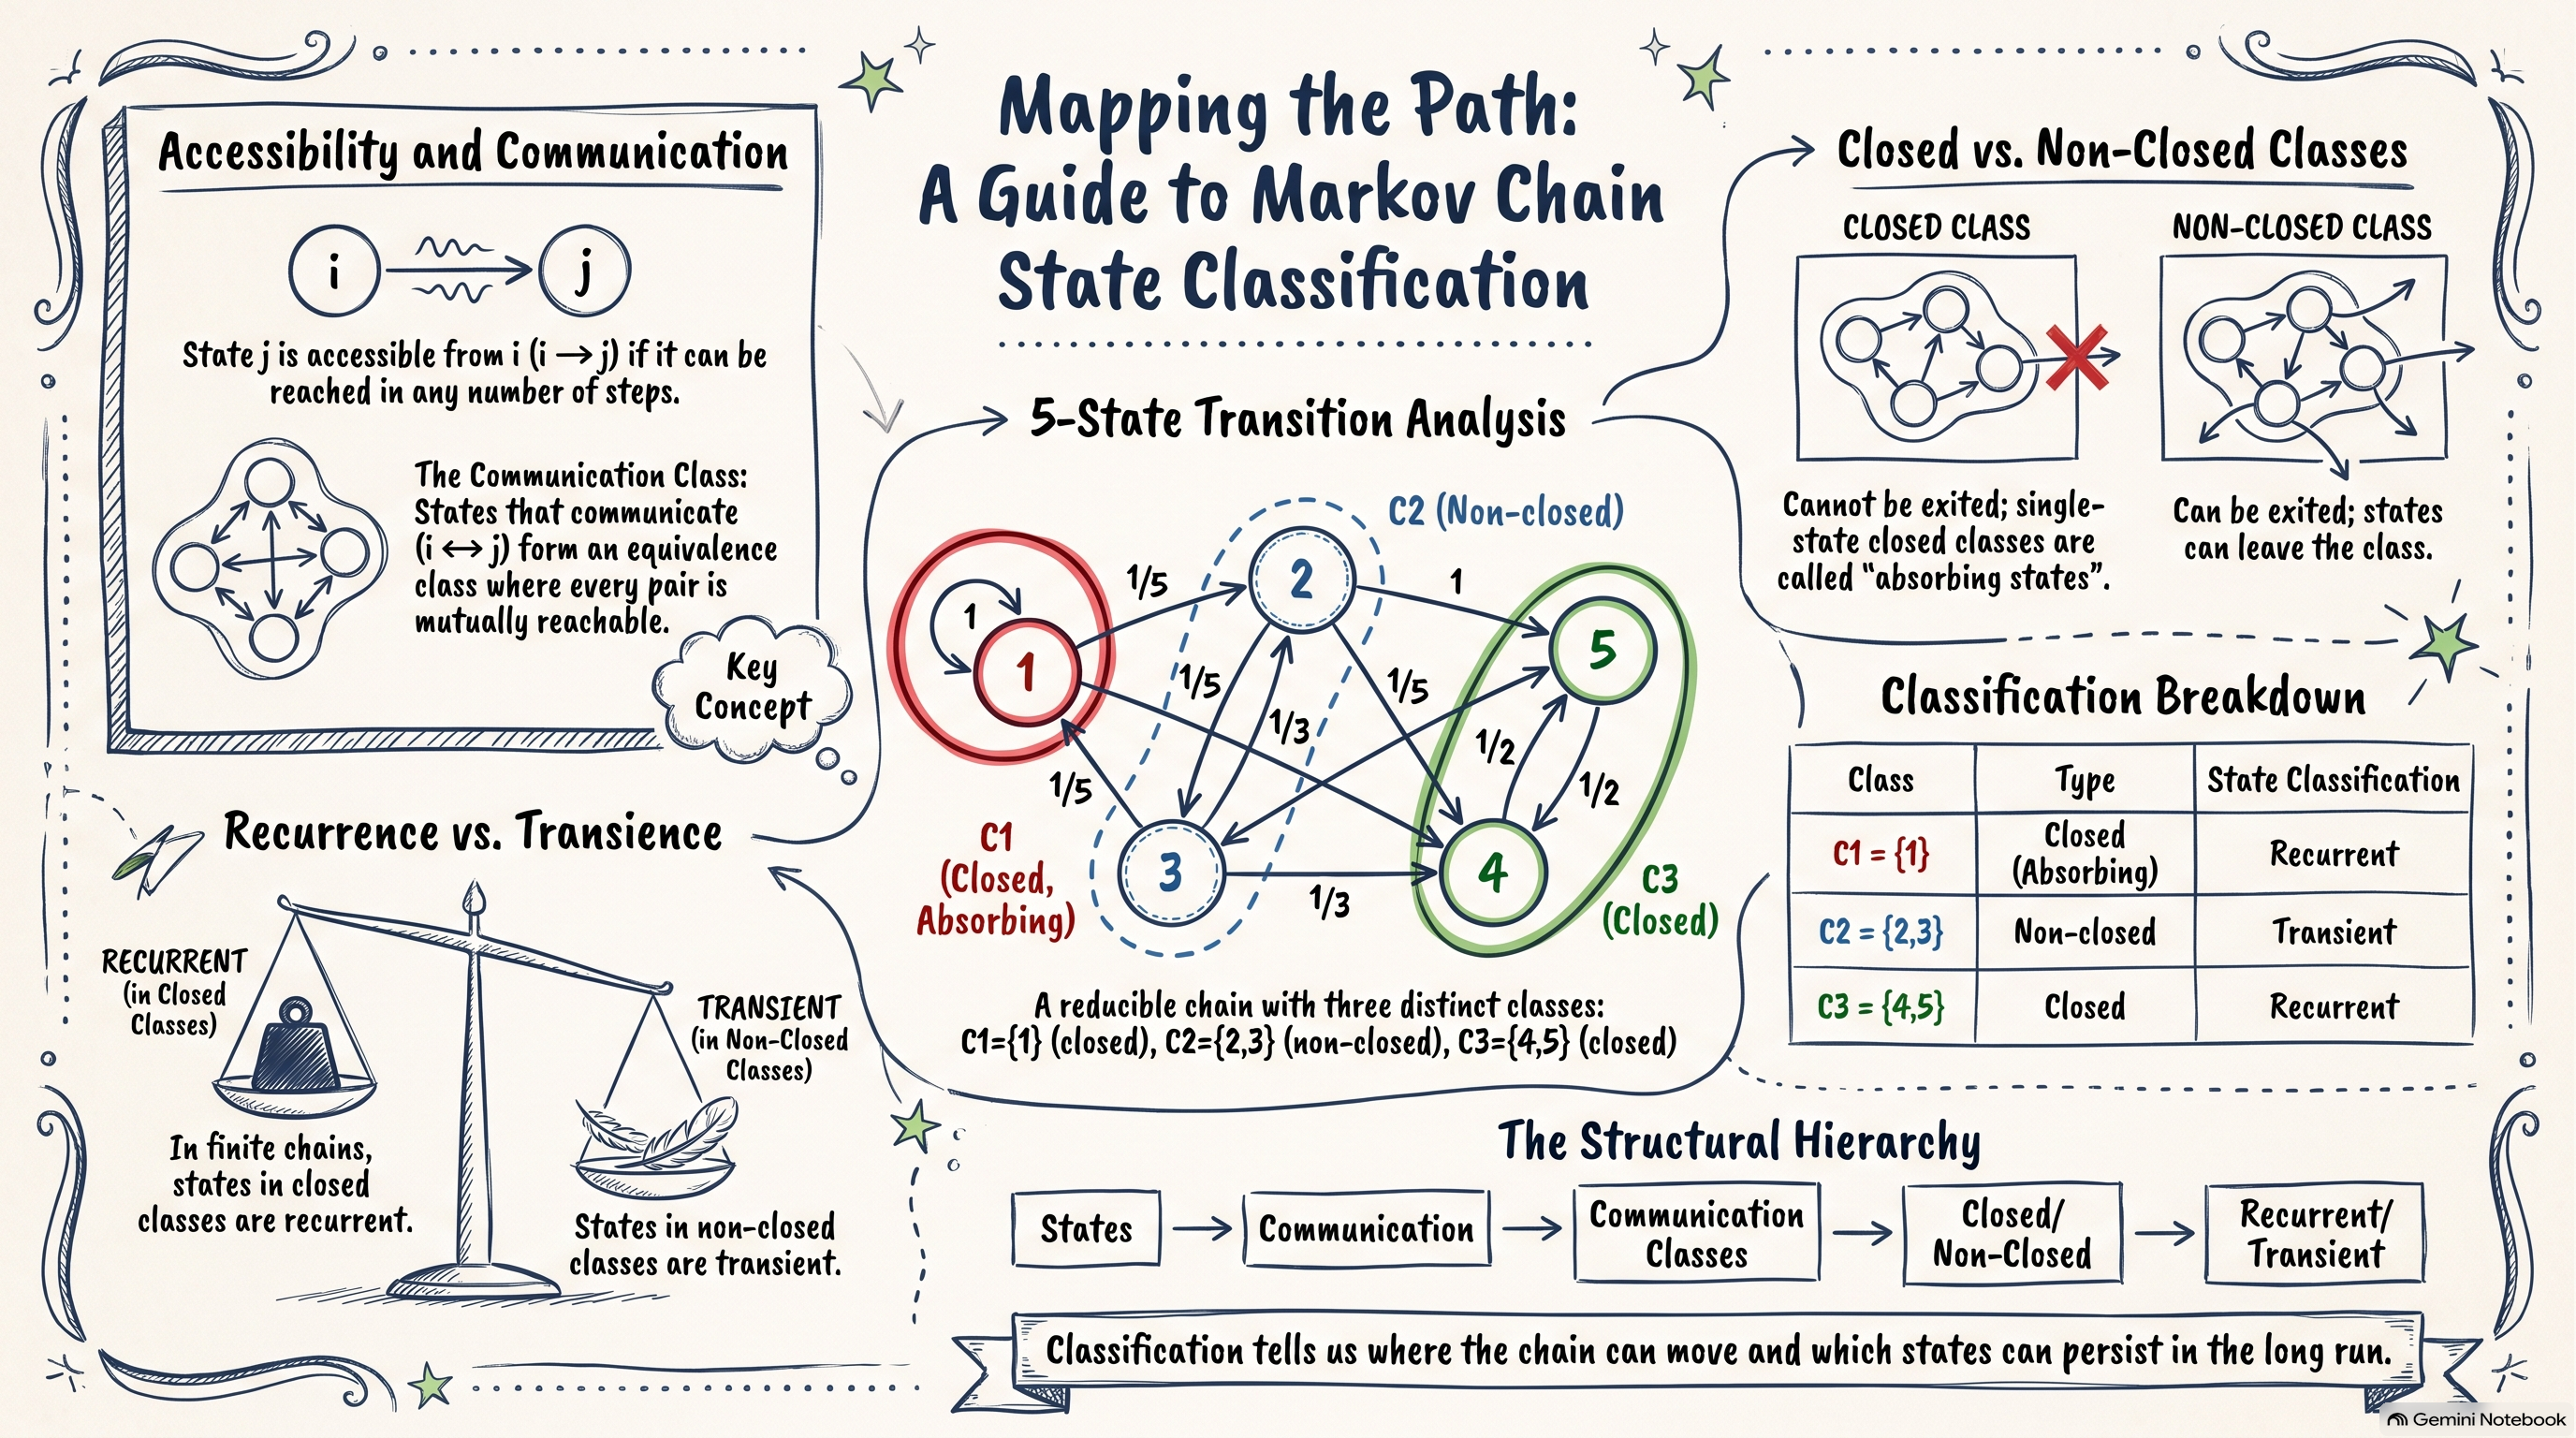
\includegraphics[width=0.75\linewidth,height=\textheight,keepaspectratio]{../figures/Markov_Chain_State_Classification_Guide.png}

}

\caption{Markov Chain State Classification Guide}

\end{figure}%
\end{frame}

\begin{frame}{Example: Communication Classes: Applications}
\protect\phantomsection\label{example-communication-classes-applications}
Consider the following three Markov chains:

\begin{enumerate}
\tightlist
\item
  an NCD system;
\item
  a health insurance system;
\item
  a simple random walk with absorbing boundaries.
\end{enumerate}

For each chain, identify the communication classes and determine whether
it is irreducible.

Use the transition diagram and transition probabilities to justify your
answers.
\end{frame}

\begin{frame}{NCD System}
\protect\phantomsection\label{ncd-system}
Suppose the states are \(\{0,1,2\}\).

Every pair of states communicates. For example, \(0\rightarrow1\) and
\(1\rightarrow0\) because \(p_{01}>0\) and \(p_{10}>0\).

Similarly, \(1\rightarrow2\) and \(2\rightarrow1\).

Hence, all states belong to one communication class: \[
\boxed{C=\{0,1,2\}}.
\]
\end{frame}

\begin{frame}{NCD System}
\protect\phantomsection\label{ncd-system-1}
Since \(C\) is the entire state space, no transition can leave the
class. Thus, \(C\) is closed.

Therefore, the Markov chain is irreducible: \[
\boxed{\text{The NCD Markov chain is irreducible.}}
\]
\end{frame}

\begin{frame}{Health Insurance System}
\protect\phantomsection\label{health-insurance-system}
The communication classes are \[
O=\{H,S\},\qquad C=\{D\}.
\]

The states \(H\) and \(S\) communicate because \(p_{HS}>0\) and
\(p_{SH}>0\).

Thus, \[
\boxed{O=\{H,S\}\text{ is a communication class}.}
\]
\end{frame}

\begin{frame}{Health Insurance System}
\protect\phantomsection\label{health-insurance-system-1}
The class \(O\) is non-closed because \(p_{HD}>0\).

The class \(C=\{D\}\) is closed because \(p_{DD}=1\). Thus, \(D\) is an
absorbing state.

Therefore, \[
\boxed{\{H,S\}\text{ is non-closed},\qquad
\{D\}\text{ is closed}.}
\]

Hence, the chain is \[
\boxed{\text{reducible}.}
\] \#\# Random Walk with Absorbing Boundaries

For a simple random walk on \(\{0,1,\ldots,N\}\) with absorbing
boundaries, the communication classes are \[
\boxed{\{1,2,\ldots,N-1\},\qquad \{0\},\qquad \{N\}.}
\]

The interior class is non-closed because the chain can move to either
boundary.
\end{frame}

\begin{frame}{Random Walk with Absorbing Boundaries}
\protect\phantomsection\label{random-walk-with-absorbing-boundaries}
The classes \(\{0\}\) and \(\{N\}\) are closed because \(0\) and \(N\)
are absorbing states.

Hence, \[
\boxed{\{1,\ldots,N-1\}\text{ is non-closed},\qquad
\{0\},\{N\}\text{ are closed}.}
\]

Therefore, the chain is \[
\boxed{\text{reducible}.}
\]
\end{frame}

\section{Absorption Probabilities in a General Markov
Chain}\label{absorption-probabilities-in-a-general-markov-chain}

\begin{frame}{From Random Walks to General Markov Chains}
\protect\phantomsection\label{from-random-walks-to-general-markov-chains}
For a random walk with absorbing barriers, we calculated the probability
of eventually reaching each absorbing state.

We now extend this idea to a \textbf{general finite Markov chain}, where
there may be several closed communication classes.

Let \(C\) be a closed communication class. Define

\[
u_i^C=\Pr(\text{eventually enter }C\mid X_0=i).
\]

Thus, \(u_i^C\) is the probability that \(C\) is the eventual
closed-class destination when the chain starts from \(i\).
\end{frame}

\begin{frame}{Boundary Conditions}
\protect\phantomsection\label{boundary-conditions}
If \(i\in C\), the chain is already in \(C\) and cannot leave:

\[
u_i^C=1.
\]

If \(i\) belongs to another closed class \(C'\neq C\), the chain cannot
move from \(C'\) to \(C\):

\[
u_i^C=0.
\]

For a transient state \(i\), condition on the state after the first
transition:

\[
u_i^C=\sum_{j\in S}p_{ij}u_j^C.
\]

This is the same \textbf{first-step analysis} used for the random walk.
\end{frame}

\begin{frame}{Matrix Formulation}
\protect\phantomsection\label{matrix-formulation}
Let \(\mathbf{u}^C=(u_1^C,\ldots,u_m^C)^\mathsf{T}\), where \(m=|S|\).

The first-step equations can be written as

\[
\boxed{\mathbf{u}^C=P\mathbf{u}^C}
\]

with boundary conditions

\[
u_i^C=
\begin{cases}
1, & i\in C,\\
0, & i\in C',\ C'\neq C,
\end{cases}
\]

for states belonging to closed classes.

The remaining equations determine the absorption probabilities for
transient states.
\end{frame}

\begin{frame}{Example: Five-State Markov Chain}
\protect\phantomsection\label{example-five-state-markov-chain}
Consider the five-state chain from the previous section:

\[
P=
\begin{bmatrix}
1&0&0&0&0\\
1/5&1/5&1/5&1/5&1/5\\
1/3&1/3&0&1/3&0\\
0&0&0&0&1\\
0&0&0&1/2&1/2
\end{bmatrix}.
\]

The closed classes are

\[
C_1=\{1\},
\qquad
C_3=\{4,5\}.
\]

Find the probability that the chain eventually enters \(C_3\), given
\(X_0=2\).
\end{frame}

\begin{frame}{Five-State Markov Chain}
\protect\phantomsection\label{five-state-markov-chain}
Define \[
u_i=\Pr(\text{eventually enter }\{4,5\}\mid X_0=i).
\]

Since \(\{4,5\}\) is closed, \[
u_4=u_5=1.
\]

Since \(\{1\}\) is another closed class, \[
u_1=0.
\]

For states \(2\) and \(3\), first-step analysis gives \[
u_2=\frac15u_2+\frac15u_3+\frac25,
\qquad
u_3=\frac13u_2+\frac13.
\]
\end{frame}

\begin{frame}{Five-State Markov Chain}
\protect\phantomsection\label{five-state-markov-chain-1}
Solving the two equations gives \[
\boxed{u_2=\frac7{11}},
\qquad
\boxed{u_3=\frac6{11}}.
\]

Therefore, \[
\boxed{
\Pr(\text{eventually enter }\{4,5\}\mid X_0=2)=\frac7{11}.
}
\]

Starting from state \(2\), the only two possible closed-class
destinations are \(\{1\}\) and \(\{4,5\}\). Hence, \[
\Pr(\text{eventually enter }\{1\}\mid X_0=2)
=1-\frac7{11}
=\frac4{11}.
\]

Thus, \[
\boxed{\frac4{11}+\frac7{11}=1.}
\]
\end{frame}

\begin{frame}{Five-State Markov Chain}
\protect\phantomsection\label{five-state-markov-chain-2}
Similarly, starting from state \(3\), \[
\boxed{
\Pr(\text{eventually enter }\{4,5\}\mid X_0=3)=\frac6{11}
}
\]

and \[
\boxed{
\Pr(\text{eventually enter }\{1\}\mid X_0=3)=\frac5{11}.
}
\]
\end{frame}

\begin{frame}{Multiple Closed Classes}
\protect\phantomsection\label{multiple-closed-classes}
Suppose a finite Markov chain has closed classes \[
C_1,C_2,\ldots,C_r.
\]

For each \(C_k\), define \[
u_i^{(k)}
=
\Pr(\text{eventually enter }C_k\mid X_0=i).
\]

For \(i\in C_k\), \[
u_i^{(k)}=1.
\]
\end{frame}

\begin{frame}{Multiple Closed Classes}
\protect\phantomsection\label{multiple-closed-classes-1}
For \(i\in C_\ell\), \(\ell\neq k\), \[
u_i^{(k)}=0.
\]

For a transient state \(i\), first-step analysis gives \[
u_i^{(k)}
=
\sum_{j\in S}p_{ij}u_j^{(k)}.
\]

Thus, the probability of eventually entering each closed class can be
found by solving these equations with the appropriate boundary
conditions.
\end{frame}

\begin{frame}{Multiple Closed Classes}
\protect\phantomsection\label{multiple-closed-classes-2}
Since a finite Markov chain eventually enters one of its closed classes
with probability \(1\),

\[
\boxed{
\sum_{k=1}^r u_i^{(k)}=1
}
\]

for every state \(i\).

Thus, the values \(u_i^{(1)},\ldots,u_i^{(r)}\) give the probabilities
of all possible long-run destinations.

For the five-state example,

\[
u_2^{(1)}=\frac4{11},
\qquad
u_2^{(3)}=\frac7{11}.
\]

Therefore, starting from state \(2\), the chain eventually enters
\({1}\) with probability \(\frac4{11}\) and \({4,5}\) with probability
\(\frac7{11}\).
\end{frame}

\begin{frame}{Key Idea}
\protect\phantomsection\label{key-idea-1}
The \textbf{closed communication classes} are the possible long-run
destinations of a finite Markov chain.

The absorption probability

\[
u_i^{(k)}
=
\Pr(\text{eventually enter }C_k\mid X_0=i)
\]

gives the probability of each destination.

Thus,

\[
\boxed{
\text{classification identifies the destinations;}
\quad
\text{first-step analysis calculates their probabilities.}
}
\]
\end{frame}

\begin{frame}{From Absorption to Long-Run Behaviour}
\protect\phantomsection\label{from-absorption-to-long-run-behaviour}
Absorption probabilities tell us \textbf{which closed class the chain
eventually enters}.

Once inside a closed class, however, the chain can continue to move
between its states.

We therefore ask:

\begin{quote}
\textbf{What does the chain do in the long run after it enters a closed
class?}
\end{quote}

This leads to the study of \textbf{stationary distributions} and
\textbf{limiting probabilities}.
\end{frame}

\section{Long-Run Behaviour of Markov
Chains}\label{long-run-behaviour-of-markov-chains}

\begin{frame}{From State Classification to Long-Run Behaviour}
\protect\phantomsection\label{from-state-classification-to-long-run-behaviour}
For a finite Markov chain, the chain eventually enters a closed
communication class with probability \(1\).

Once inside, it cannot leave but can continue moving between states.

We therefore ask:

\begin{quote}
\textbf{What happens to the distribution of the chain as
\(n\rightarrow\infty\)?}
\end{quote}

We will study:

\begin{itemize}
\tightlist
\item
  \textbf{stationary distributions} --- distributions unchanged by each
  transition;
\item
  \textbf{limiting distributions} --- distributions approached as
  \(n\rightarrow\infty\);
\item
  \textbf{periodicity} --- a structural property that can prevent
  convergence.
\end{itemize}

A stationary distribution describes \textbf{equilibrium}, whereas a
limiting distribution describes \textbf{what the chain approaches over
time}.
\end{frame}

\begin{frame}{Stationary vs.~Limiting Distributions}
\protect\phantomsection\label{stationary-vs.-limiting-distributions}
\begin{figure}[H]

{\centering 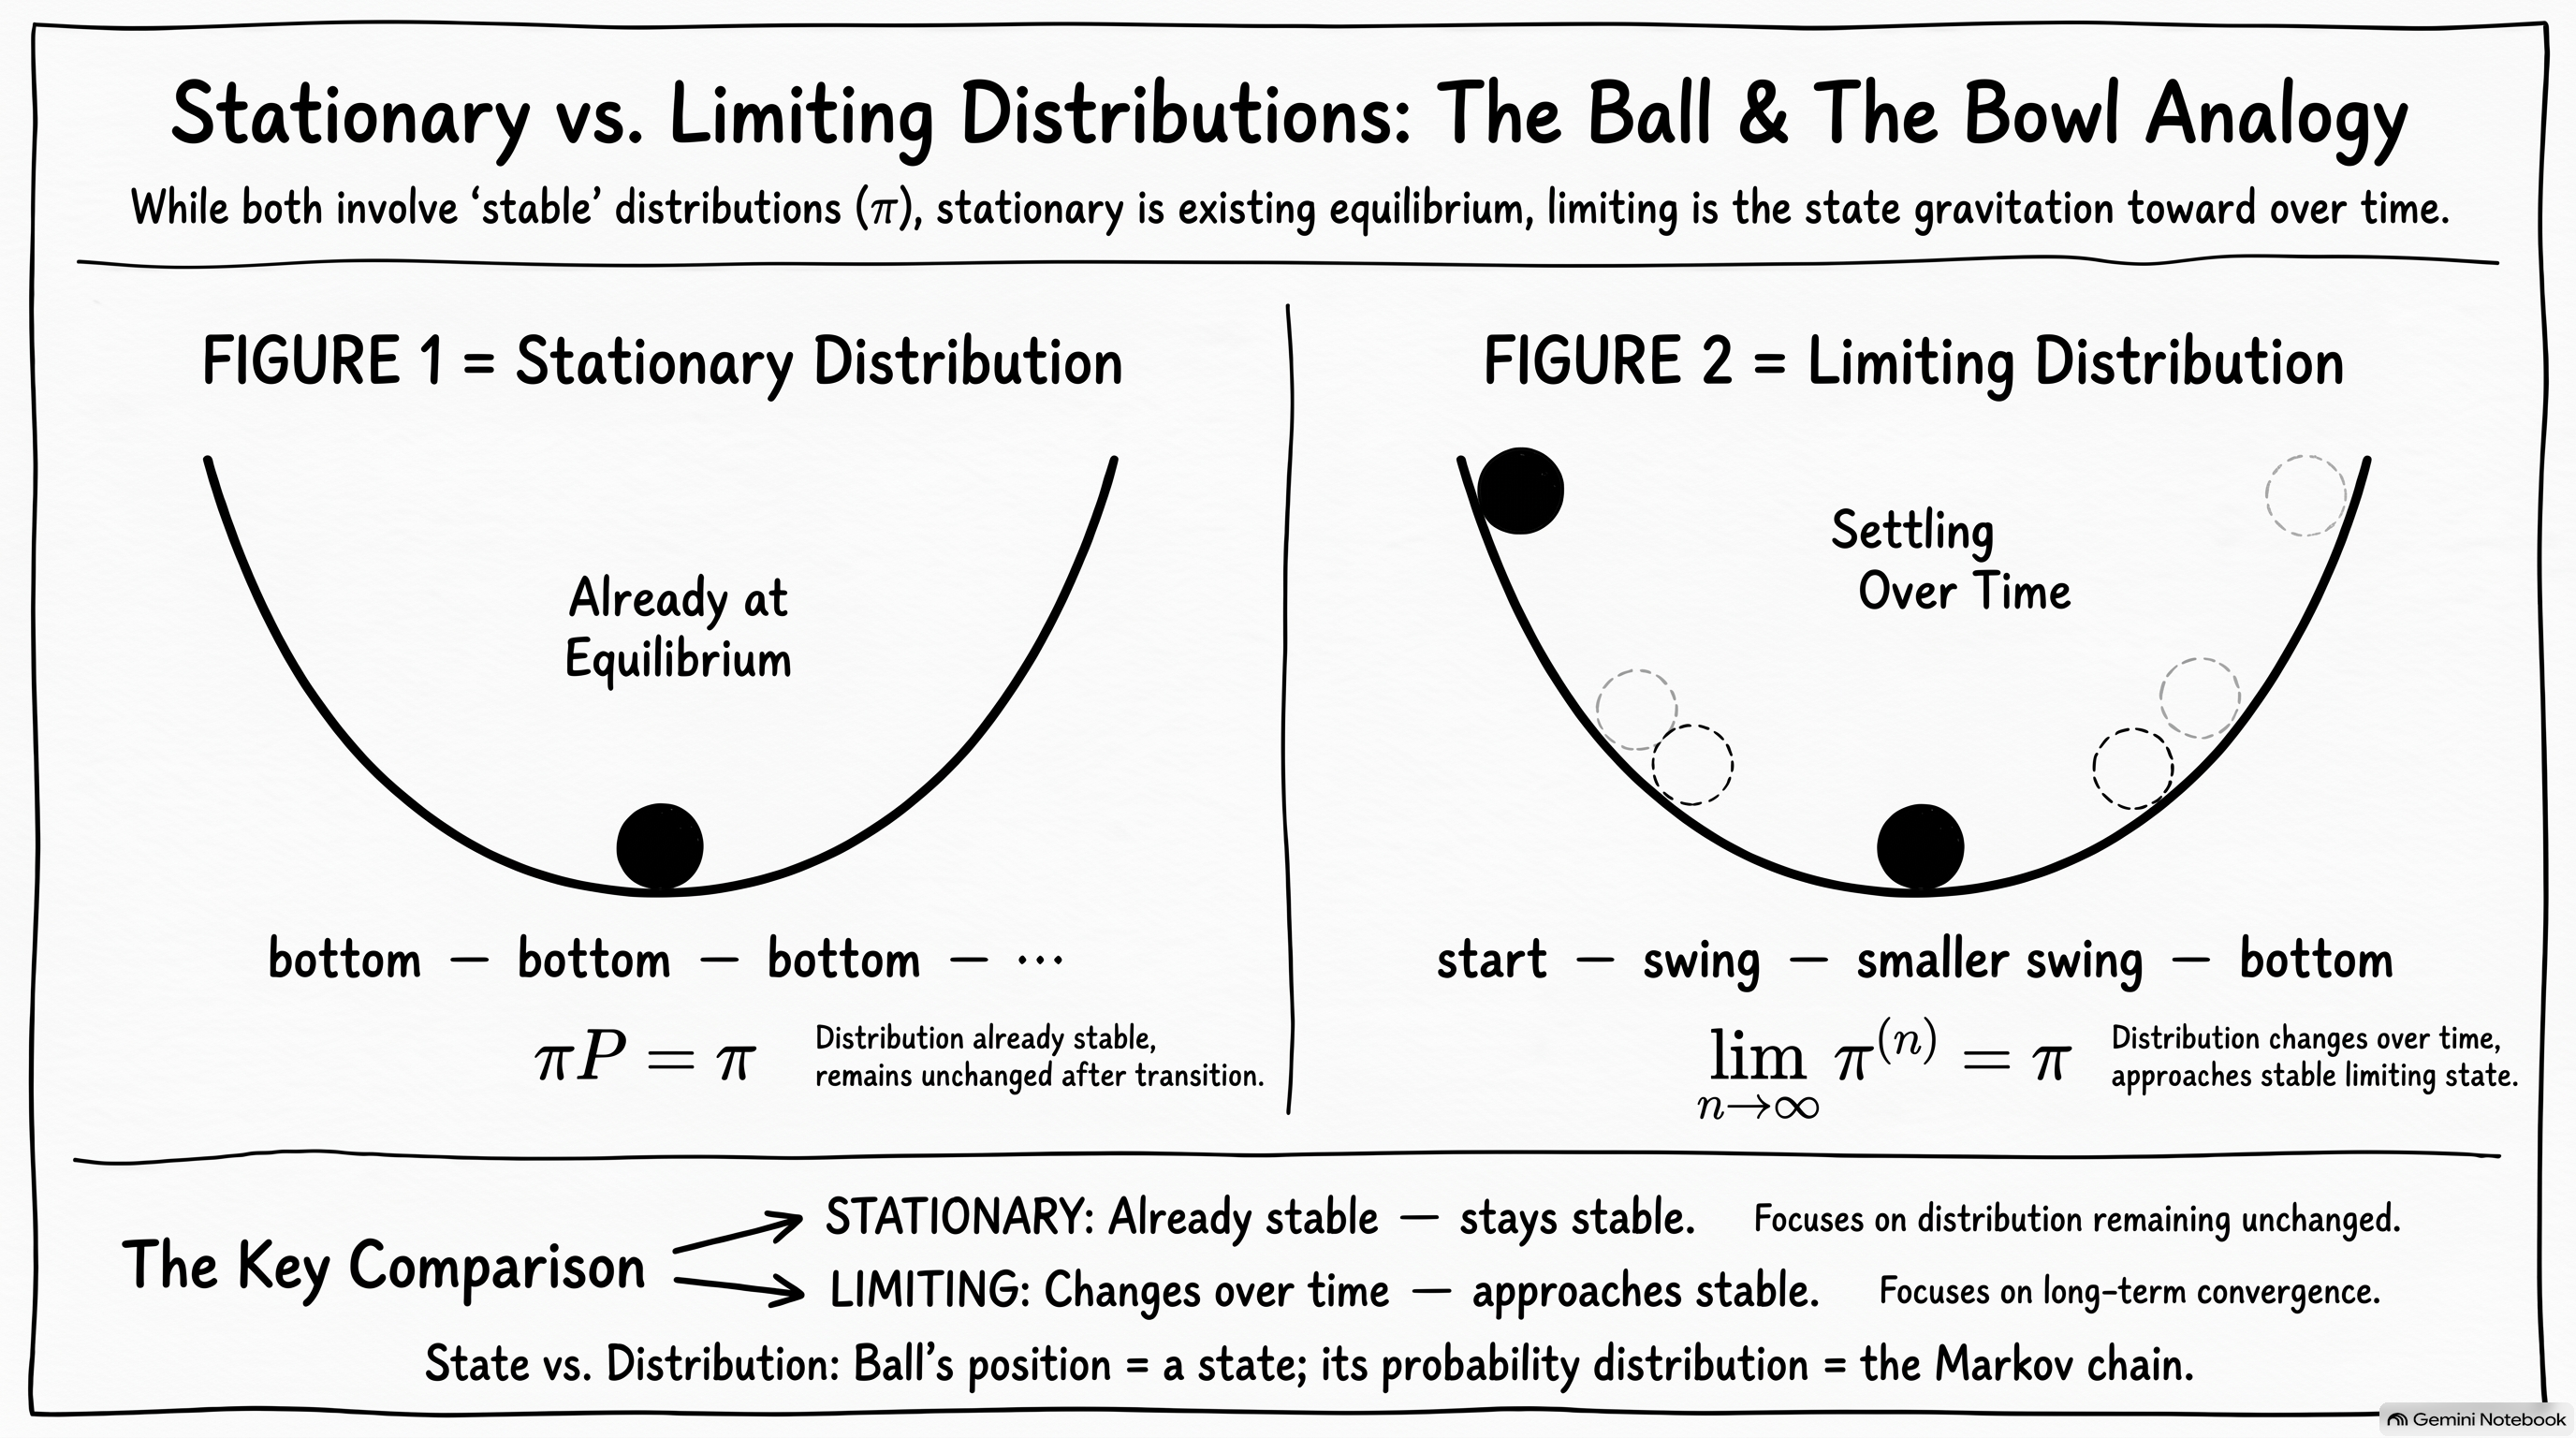
\includegraphics[width=0.75\linewidth,height=\textheight,keepaspectratio]{../figures/Stationary_vs._Limiting_Distributions_Analogy.png}

}

\caption{Stationary vs.~Limiting Distributions Analogy}

\end{figure}%
\end{frame}

\begin{frame}{Within a Closed Communicating Class}
\protect\phantomsection\label{within-a-closed-communicating-class}
Suppose \(C\) is a closed communicating class.

\[
\text{enter }C
\quad\longrightarrow\quad
\text{remain in }C
\quad\longrightarrow\quad
\text{continue moving within }C
\]

Once the chain enters \(C\), it cannot leave. The chain therefore
continues to move among the states in \(C\).
\end{frame}

\begin{frame}{Within a Closed Communicating Class}
\protect\phantomsection\label{within-a-closed-communicating-class-1}
For a finite closed communicating class, there is a unique stationary
probability distribution \[
\boldsymbol{\pi}=(\pi_i)_{i\in C}
\] satisfying \[
\boldsymbol{\pi}P_C=\boldsymbol{\pi},
\qquad
\pi_i\geq0,
\qquad
\sum_{i\in C}\pi_i=1.
\]

Here, \(P_C\) is the transition matrix restricted to the states in
\(C\).
\end{frame}

\begin{frame}{Within a Closed Communicating Class}
\protect\phantomsection\label{within-a-closed-communicating-class-2}
If the chain starts with distribution \(\boldsymbol{\pi}\), then \[
\boldsymbol{\pi}P_C^n=\boldsymbol{\pi},
\qquad n\geq1.
\]

Thus, \(\boldsymbol{\pi}\) describes an \textbf{equilibrium distribution
within the closed class}.

It gives the long-run proportions associated with the states in \(C\),
provided the chain is aperiodic.
\end{frame}

\begin{frame}{Stationary Distributions}
\protect\phantomsection\label{stationary-distributions}
Consider a Markov chain with transition matrix \(P\) and state space
\(S\).

A probability distribution \(\boldsymbol{\pi}=(\pi_i)_{i\in S}\) is
\textbf{stationary} if

\[
\boxed{\boldsymbol{\pi}P=\boldsymbol{\pi}.}
\]

Equivalently, for each \(j\in S\),

\[
\pi_j=\sum_{i\in S}\pi_i p_{ij}.
\]

The components satisfy

\[
\pi_i\geq0,
\qquad
\sum_{i\in S}\pi_i=1.
\]
\end{frame}

\begin{frame}{Stationary Distributions}
\protect\phantomsection\label{stationary-distributions-1}
The equation \(\boldsymbol{\pi}P=\boldsymbol{\pi}\) means that the
distribution is unchanged after one transition.

Consequently,

\[
\boxed{\boldsymbol{\pi}P^n=\boldsymbol{\pi},\qquad n\geq1.}
\]

For a finite irreducible Markov chain, the stationary distribution
exists and is unique.
\end{frame}

\begin{frame}{Example: Finding a Stationary Distribution}
\protect\phantomsection\label{example-finding-a-stationary-distribution}
Consider

\[
P=
\begin{bmatrix}
1-a&a\\
b&1-b
\end{bmatrix},
\qquad 0<a,b<1.
\]

Let \(\boldsymbol{\pi}=(\pi_0,\pi_1)\).

From \(\boldsymbol{\pi}P=\boldsymbol{\pi}\),

\[
\pi_0(1-a)+\pi_1b=\pi_0
\quad\Longrightarrow\quad
a\pi_0=b\pi_1.
\]
\end{frame}

\begin{frame}{Example: Finding a Stationary Distribution}
\protect\phantomsection\label{example-finding-a-stationary-distribution-1}
Together with \(\pi_0+\pi_1=1\),

\[
\boxed{
\pi_0=\frac{b}{a+b},
\qquad
\pi_1=\frac{a}{a+b}.
}
\]

Hence,

\[
\boxed{
\boldsymbol{\pi}
=
\left(
\frac{b}{a+b},
\frac{a}{a+b}
\right).
}
\]

For \(a=0.2\) and \(b=0.4\),

\[
\boxed{\boldsymbol{\pi}=\left(\frac23,\frac13\right).}
\]
\end{frame}

\begin{frame}{Stationary Distribution: Interpretation}
\protect\phantomsection\label{stationary-distribution-interpretation}
A stationary distribution is an \textbf{equilibrium distribution}.

If

\[
\boldsymbol{\pi}=(2/3,1/3),
\]

then a chain starting with this distribution remains distributed as
\((2/3,1/3)\) after every transition.

It does \textbf{not} mean that an individual chain remains in one state.
\end{frame}

\begin{frame}{Stationary Distribution: Interpretation}
\protect\phantomsection\label{stationary-distribution-interpretation-1}
The individual chain continues to move:

\[
0\longrightarrow1\longrightarrow0\longrightarrow0\longrightarrow1\longrightarrow\cdots
\]

while the \textbf{distribution across many chains} remains unchanged.

This distinction is important when interpreting stationary distributions
in applications such as NCD systems.
\end{frame}

\begin{frame}{Limiting Distributions}
\protect\phantomsection\label{limiting-distributions}
A \textbf{limiting distribution} describes the distribution approached
by the chain after a large number of transitions.

For \(i,j\in S\), suppose

\[
\boxed{
\lim_{n\rightarrow\infty}p_{ij}^{(n)}=\pi_j.
}
\]

The limit depends on the destination state \(j\), but not on the initial
state \(i\).

Thus, for large \(n\), the probability of being in state \(j\) is
approximately \(\pi_j\), regardless of where the chain started.
\end{frame}

\begin{frame}{Limiting Behaviour of \(P^n\)}
\protect\phantomsection\label{limiting-behaviour-of-pn}
Recall that

\[
P^n=
\begin{bmatrix}
p_{11}^{(n)}&p_{12}^{(n)}&\cdots\\
p_{21}^{(n)}&p_{22}^{(n)}&\cdots\\
\vdots&\vdots&\ddots
\end{bmatrix}.
\]

If \(p_{ij}^{(n)}\longrightarrow\pi_j\) for every \(i,j\), then every
row of \(P^n\) approaches the same distribution:

\[
\boxed{
P^n
\longrightarrow
\begin{bmatrix}
\boldsymbol{\pi}\\
\boldsymbol{\pi}\\
\vdots\\
\boldsymbol{\pi}
\end{bmatrix}.
}
\]
\end{frame}

\begin{frame}{Limiting Behaviour of \(P^n\)}
\protect\phantomsection\label{limiting-behaviour-of-pn-1}
Equivalently,

\[
\boxed{
P^n\longrightarrow\boldsymbol{1}\boldsymbol{\pi}.
}
\]

Hence, for large \(n\), the distribution of the chain becomes
independent of its initial state.
\end{frame}

\begin{frame}{Initial Distribution}
\protect\phantomsection\label{initial-distribution}
Suppose the initial distribution is

\[
\boldsymbol{\pi}^{(0)}
=
\left(\Pr(X_0=i)\right)_{i\in S}.
\]

After \(n\) transitions,

\[
\boxed{
\boldsymbol{\pi}^{(n)}
=
\boldsymbol{\pi}^{(0)}P^n.
}
\]

If

\[
P^n\longrightarrow\boldsymbol{1}\boldsymbol{\pi},
\]

then

\[
\begin{aligned}
\boldsymbol{\pi}^{(n)}
&\longrightarrow
\boldsymbol{\pi}^{(0)}
\boldsymbol{1}\boldsymbol{\pi}\\
&=\boldsymbol{\pi},
\end{aligned}
\]

because \(\boldsymbol{\pi}^{(0)}\boldsymbol{1}=1\).
\end{frame}

\begin{frame}{Initial Distribution}
\protect\phantomsection\label{initial-distribution-1}
Thus,

\[
\boxed{
\boldsymbol{\pi}^{(n)}
\longrightarrow\boldsymbol{\pi}.
}
\]

The limiting distribution is independent of the initial distribution.
\end{frame}

\begin{frame}{Stationary vs.~Limiting Distributions}
\protect\phantomsection\label{stationary-vs.-limiting-distributions-1}
The two concepts answer different questions.

{\def\LTcaptype{none} % do not increment counter
\begin{longtable}[]{@{}
  >{\raggedright\arraybackslash}p{(\linewidth - 4\tabcolsep) * \real{0.1505}}
  >{\raggedright\arraybackslash}p{(\linewidth - 4\tabcolsep) * \real{0.3871}}
  >{\raggedright\arraybackslash}p{(\linewidth - 4\tabcolsep) * \real{0.4624}}@{}}
\toprule\noalign{}
\begin{minipage}[b]{\linewidth}\raggedright
\end{minipage} & \begin{minipage}[b]{\linewidth}\raggedright
Stationary distribution
\end{minipage} & \begin{minipage}[b]{\linewidth}\raggedright
Limiting distribution
\end{minipage} \\
\midrule\noalign{}
\endhead
Question & Is the distribution unchanged? & What distribution is
approached? \\
Condition & \(\boldsymbol{\pi}P=\boldsymbol{\pi}\) &
\(\boldsymbol{\pi}^{(n)}\to\boldsymbol{\pi}\) \\
Interpretation & Equilibrium & Long-run distribution \\
\bottomrule\noalign{}
\end{longtable}
}

If a limiting distribution exists, it must be stationary:

\[
\boxed{
\text{limiting distribution}
\Longrightarrow
\text{stationary distribution}.
}
\]
\end{frame}

\begin{frame}{Stationary vs.~Limiting Distributions}
\protect\phantomsection\label{stationary-vs.-limiting-distributions-2}
However,

\[
\boxed{
\text{stationary distribution}
\not\Longrightarrow
\text{limiting distribution}.
}
\]

Periodicity can prevent convergence.
\end{frame}

\begin{frame}{Example: A Stationary but Non-Limiting Distribution}
\protect\phantomsection\label{example-a-stationary-but-non-limiting-distribution}
Consider

\[
P=
\begin{bmatrix}
0&1\\
1&0
\end{bmatrix}.
\]

The stationary distribution is

\[
\boldsymbol{\pi}
=
\left(\frac12,\frac12\right).
\]

However, if \(X_0=0\),

\[
\boldsymbol{\pi}^{(0)}=(1,0),
\]

and the distributions alternate:

\[
(1,0),\quad
(0,1),\quad
(1,0),\quad
(0,1),\quad\ldots
\]
\end{frame}

\begin{frame}{Example: A Stationary but Non-Limiting Distribution}
\protect\phantomsection\label{example-a-stationary-but-non-limiting-distribution-1}
Therefore, \(\boldsymbol{\pi}^{(n)}\) does not converge.

The chain is \textbf{periodic}, with period \(2\).
\end{frame}

\begin{frame}{Conditions for Convergence}
\protect\phantomsection\label{conditions-for-convergence}
For a finite irreducible Markov chain:

\begin{itemize}
\tightlist
\item
  a stationary distribution exists and is unique;
\item
  \textbf{aperiodicity} is required for convergence to that
  distribution.
\end{itemize}

If the chain is finite, irreducible, and aperiodic, then

\[
\boxed{
p_{ij}^{(n)}
\longrightarrow
\pi_j
\qquad\text{for all }i,j.
}
\]
\end{frame}

\begin{frame}{Conditions for Convergence}
\protect\phantomsection\label{conditions-for-convergence-1}
Equivalently, for any initial distribution,

\[
\boxed{
\boldsymbol{\pi}^{(0)}P^n
\longrightarrow
\boldsymbol{\pi}.
}
\]

Thus,

\[
\boxed{
\text{finite}
+\text{ irreducible}
+\text{ aperiodic}
\Longrightarrow
\text{convergence to a unique stationary distribution}.
}
\]
\end{frame}

\begin{frame}{Periodicity}
\protect\phantomsection\label{periodicity}
A state \(i\) has \textbf{period}

\[
d(i)
=
\gcd\{n\geq1:p_{ii}^{(n)}>0\}.
\]

If

\[
d(i)=1,
\]

then state \(i\) is \textbf{aperiodic}.

For an irreducible chain, all states have the same period, so the chain
itself can be described as periodic or aperiodic.
\end{frame}

\begin{frame}{Periodicity}
\protect\phantomsection\label{periodicity-1}
The key question is:

\begin{quote}
\textbf{Do the possible return times have a common divisor greater than
\(1\)?}
\end{quote}
\end{frame}

\begin{frame}{Example: Aperiodicity in an NCD System}
\protect\phantomsection\label{example-aperiodicity-in-an-ncd-system}
Consider the four-state NCD system

\[
P=
\begin{bmatrix}
0.80&0.20&0&0\\
0.10&0.80&0.10&0\\
0&0.10&0.80&0.10\\
0&0&0.20&0.80
\end{bmatrix}.
\]

The chain is irreducible because every state can be reached from every
other state.

Also,

\[
p_{ii}>0
\qquad\text{for every }i.
\]
\end{frame}

\begin{frame}{Example: Aperiodicity in an NCD System}
\protect\phantomsection\label{example-aperiodicity-in-an-ncd-system-1}
For example,

\[
p_{22}=0.80>0.
\]

Therefore, a return after one transition is possible:

\[
p_{22}^{(1)}>0.
\]

Hence,

\[
d(2)=1.
\]

Since the chain is irreducible, all states are aperiodic.

Thus, the NCD system is

\[
\boxed{\text{irreducible and aperiodic}.}
\]
\end{frame}

\begin{frame}{Checking Aperiodicity}
\protect\phantomsection\label{checking-aperiodicity}
There are several useful ways to identify aperiodicity.

\textbf{Self-loop:} If

\[
p_{ii}>0,
\]

then \(p_{ii}^{(1)}>0\), so

\[
d(i)=1.
\]
\end{frame}

\begin{frame}{Checking Aperiodicity}
\protect\phantomsection\label{checking-aperiodicity-1}
\textbf{Two return times:} If

\[
p_{ii}^{(m)}>0,\qquad
p_{ii}^{(n)}>0,
\qquad
\gcd(m,n)=1,
\]

then

\[
d(i)=1.
\]

For an irreducible chain, if one state is aperiodic, then every state is
aperiodic.
\end{frame}

\begin{frame}{Example: Two Return Times with GCD \(1\)}
\protect\phantomsection\label{example-two-return-times-with-gcd-1}
Suppose returns to state \(2\) are possible after \(2\) and \(3\)
transitions:

\[
p_{22}^{(2)}>0,
\qquad
p_{22}^{(3)}>0.
\]

Then

\[
d(2)
=
\gcd\{n\geq1:p_{22}^{(n)}>0\}
\leq
\gcd(2,3)=1.
\]

Therefore,

\[
\boxed{d(2)=1,}
\]

so state \(2\) is aperiodic.

A self-loop is \textbf{not necessary} for aperiodicity.
\end{frame}

\begin{frame}{Example: Period \(2\)}
\protect\phantomsection\label{example-period-2}
Consider

\[
P=
\begin{bmatrix}
0&1/2&0&1/2\\
1/4&0&3/4&0\\
0&1/3&0&2/3\\
1/2&0&1/2&0
\end{bmatrix}.
\]

The states split into two groups:

\[
\{1,3\}
\qquad\text{and}\qquad
\{2,4\}.
\]
\end{frame}

\begin{frame}{Example: Period \(2\)}
\protect\phantomsection\label{example-period-2-1}
Every transition moves between the two groups:

\[
\{1,3\}
\longrightarrow
\{2,4\}
\longrightarrow
\{1,3\}
\longrightarrow\cdots
\]

Therefore, a return to the original state is possible only after an even
number of transitions.

Hence,

\[
p_{ii}^{(2n)}>0,
\qquad
p_{ii}^{(2n+1)}=0,
\]

and

\[
\boxed{d(i)=2.}
\]

The chain is periodic.
\end{frame}

\begin{frame}{Why Aperiodicity Matters}
\protect\phantomsection\label{why-aperiodicity-matters}
A periodic chain can continue to visit every state indefinitely while
its probabilities oscillate.

For example,

\[
P=
\begin{bmatrix}
0&1\\
1&0
\end{bmatrix}
\]

has stationary distribution

\[
\left(\frac12,\frac12\right),
\]

but its distribution alternates between

\[
(1,0)
\quad\text{and}\quad
(0,1).
\]
\end{frame}

\begin{frame}{Why Aperiodicity Matters}
\protect\phantomsection\label{why-aperiodicity-matters-1}
Aperiodicity removes this persistent oscillation.

Thus, for a finite irreducible aperiodic chain,

\[
\boxed{
p_{ij}^{(n)}
\longrightarrow
\pi_j.
}
\]
\end{frame}

\begin{frame}{Example: Convergence to a Limiting Distribution}
\protect\phantomsection\label{example-convergence-to-a-limiting-distribution}
Consider

\[
P=
\begin{bmatrix}
1/3&2/3\\
2/3&1/3
\end{bmatrix}.
\]

The chain is irreducible and aperiodic because

\[
p_{01}>0,\qquad p_{00}>0.
\]

Its stationary distribution is

\[
\boldsymbol{\pi}
=
\left(\frac12,\frac12\right).
\]
\end{frame}

\begin{frame}{Example: Convergence to a Limiting Distribution}
\protect\phantomsection\label{example-convergence-to-a-limiting-distribution-1}
Starting from state \(0\), \[
\boldsymbol{\pi}^{(0)}=(1,0).
\]

After one transition, \[
\boldsymbol{\pi}^{(1)}
=
\left(\frac13,\frac23\right),
\]

and after two transitions, \[
\boldsymbol{\pi}^{(2)}
=
\left(\frac59,\frac49\right).
\]
\end{frame}

\begin{frame}{Example: Convergence to a Limiting Distribution}
\protect\phantomsection\label{example-convergence-to-a-limiting-distribution-2}
As \(n\) increases, \[
\boxed{
\boldsymbol{\pi}^{(n)}
\longrightarrow
\left(\frac12,\frac12\right).
}
\]

The same limiting distribution is obtained from any initial
distribution.
\end{frame}

\begin{frame}{Long-Run Behaviour: Summary}
\protect\phantomsection\label{long-run-behaviour-summary}
For a finite Markov chain:

\[
\boxed{
\begin{array}{c}
\text{irreducible}\\
+\ \text{aperiodic}
\end{array}
}
\quad\Longrightarrow\quad
\boxed{
\begin{array}{c}
\text{unique stationary distribution}\\
\boldsymbol{\pi}P=\boldsymbol{\pi}\\[2pt]
\text{limiting distribution}\\
\boldsymbol{\pi}^{(0)}P^n\to\boldsymbol{\pi}
\end{array}
}
\]
\end{frame}

\begin{frame}{Long-Run Behaviour: Summary}
\protect\phantomsection\label{long-run-behaviour-summary-1}
The roles of the conditions are:

\begin{itemize}
\tightlist
\item
  \textbf{irreducibility:} all states communicate;
\item
  \textbf{aperiodicity:} prevents persistent oscillation;
\item
  \textbf{finiteness:} ensures the stationary distribution exists for an
  irreducible chain.
\end{itemize}

Thus, the stationary distribution describes \textbf{equilibrium}, while
the limiting distribution describes \textbf{convergence to equilibrium}.
\end{frame}

\begin{frame}{Application: Long-Run Behaviour of an NCD System}
\protect\phantomsection\label{application-long-run-behaviour-of-an-ncd-system}
Consider an NCD system with three levels:

{\def\LTcaptype{none} % do not increment counter
\begin{longtable}[]{@{}lrrr@{}}
\toprule\noalign{}
Level & 1 & 2 & 3 \\
\midrule\noalign{}
\endhead
Discount & \(0%
\) & \(30%
\) & \(50%
\) \\
\bottomrule\noalign{}
\end{longtable}
}

Suppose:

\begin{itemize}
\tightlist
\item
  no claim \(\rightarrow\) move one level higher, or remain at level 3;
\item
  one claim \(\rightarrow\) move one level lower, or remain at level 1;
\item
  two or more claims \(\rightarrow\) move to level 1.
\end{itemize}
\end{frame}

\begin{frame}{Application: Long-Run Behaviour of an NCD System}
\protect\phantomsection\label{application-long-run-behaviour-of-an-ncd-system-1}
For \(N\sim\operatorname{Poisson}(\lambda)\), define

\[
q_0=\Pr(N=0),\qquad
q_1=\Pr(N=1),\qquad
q_2=\Pr(N\geq2).
\]

Then

\[
q_0=e^{-\lambda},
\qquad
q_1=\lambda e^{-\lambda},
\qquad
q_2=1-q_0-q_1.
\]

The transition matrix is

\[
\boxed{
P=
\begin{bmatrix}
q_1+q_2&q_0&0\\
1-q_0&0&q_0\\
q_2&q_1&q_0
\end{bmatrix}.
}
\]
\end{frame}

\begin{frame}{Application: Long-Run NCD Distribution}
\protect\phantomsection\label{application-long-run-ncd-distribution}
Let

\[
\boldsymbol{\pi}
=
(\pi_1,\pi_2,\pi_3)
\]

be the stationary distribution.

It satisfies

\[
\boldsymbol{\pi}P=\boldsymbol{\pi},
\qquad
\pi_1+\pi_2+\pi_3=1.
\]

For a portfolio of 5,000 policyholders, the long-run expected numbers at
the three levels are

\[
\boxed{
(5000\pi_1,\;5000\pi_2,\;5000\pi_3).
}
\]
\end{frame}

\begin{frame}{Application: Long-Run NCD Distribution}
\protect\phantomsection\label{application-long-run-ncd-distribution-1}
If the full premium is \(B\), the long-run expected premium per driver
is

\[
\boxed{
B(\pi_1+0.70\pi_2+0.50\pi_3).
}
\]

Thus, the stationary distribution connects the Markov-chain model
directly to the long-run composition and premium income of the insurance
portfolio.
\end{frame}

\begin{frame}{Long-Run Behaviour with Several Closed Classes}
\protect\phantomsection\label{long-run-behaviour-with-several-closed-classes}
If a finite chain has several closed communication classes, there need
not be a single limiting distribution independent of the initial state.

The chain first enters one of the closed classes, with probabilities
determined by the \textbf{absorption probabilities} studied earlier.
\end{frame}

\begin{frame}{Long-Run Behaviour with Several Closed Classes}
\protect\phantomsection\label{long-run-behaviour-with-several-closed-classes-1}
Once inside a closed class, its long-run behaviour is determined by the
stationary distribution of that class.

Thus,

\[
\boxed{
\text{absorption probabilities}
\quad+\quad
\text{within-class stationary distributions}
}
\]

determine the long-run behaviour of a reducible finite Markov chain.
\end{frame}




\end{document}
